\documentclass{beamer}

\usepackage{amsmath}
\usepackage{amssymb}

\usepackage{tikz}
\usetikzlibrary{positioning}

\title{Set}
\author{Neeraj Varghese}
\date{\today}

\begin{document}


\begin{frame}
    \titlepage
\end{frame}


\begin{frame}{Mathematical Form (1--5)}
\footnotesize

\textbf{1.} $\{1,2,3,4,5,6\}$\\
$X=\{x:x\in\mathbb N,\;1\le x\le6\}$

\vspace{0.1cm}

\textbf{2.} $\{2,4,6,8,10\}$\\
$X=\{x:x\in\mathbb N,\;x\equiv0\pmod2,\;2\le x\le10\}$

\vspace{0.1cm}

\textbf{3.} $\{1,3,5,7,9\}$\\
$X=\{x:x\in\mathbb N,\;x\equiv1\pmod2,\;1\le x\le9\}$

\vspace{0.1cm}

\textbf{4.} $\{5,10,15,20,25\}$\\
$X=\{x:x=5n,\;1\le n\le5,\;n\in\mathbb N\}$

\vspace{0.1cm}

\textbf{5.} $\{1,4,9,16,25\}$\\
$X=\{x:x=n^2,\;1\le n\le5,\;n\in\mathbb N\}$

\end{frame}

%---------------- Slide 2 ----------------%
\begin{frame}{Mathematical Form (6--10)}
\footnotesize

\textbf{6.} $\{1,8,27,64,125\}$\\
$X=\{x:x=n^3,\;1\le n\le5,\;n\in\mathbb N\}$

\vspace{0.1cm}

\textbf{7.} $\{2,3,5,7,11\}$\\
$X=\{x:x\text{ is prime},\;2\le x\le11\}$

\vspace{0.1cm}

\textbf{8.} $\{10,20,30,40,50\}$\\
$X=\{x:x=10n,\;1\le n\le5,\;n\in\mathbb N\}$

\vspace{0.1cm}

\textbf{9.} $\{3,6,9,12,15\}$\\
$X=\{x:x=3n,\;1\le n\le5,\;n\in\mathbb N\}$

\vspace{0.1cm}

\textbf{10.} $\{0,1,2,3,4,5\}$\\
$X=\{x:x\in\mathbb Z,\;0\le x\le5\}$

\end{frame}
\begin{frame}{General Inclusion--Exclusion Principle}
\small

For finite sets $A_1,A_2,\ldots,A_n$,

\[
\begin{aligned}
|A_1\cup A_2\cup\cdots\cup A_n|
&=\sum_{i=1}^{n}|A_i| \\
&\quad-\sum_{1\le i<j\le n}|A_i\cap A_j| \\
&\quad+\sum_{1\le i<j<k\le n}
|A_i\cap A_j\cap A_k| \\
&\quad-\cdots \\
&\quad+(-1)^{n-1}
|A_1\cap A_2\cap\cdots\cap A_n|.
\end{aligned}
\]

\vspace{0.3cm}


\end{frame}
\begin{frame}{Cardinality of a Set \& Finite Set}

\textbf{Cardinality of a Set}

The cardinality of a set is the number of distinct elements in the set.
It is denoted by $|A|$.

\textbf{Example }

\[
A=\{\text{Python},\text{R},\text{SQL},\text{TensorFlow}\}
\]

\[
|A|=4
\]

\vspace{0.2cm}

\textbf{Finite Set}

A finite set contains a limited number of elements.

\[
B=\{\text{CNN},\text{RNN},\text{Transformer},\text{GAN}\}
\]

Since

\[
|B|=4,
\]

$B$ is a finite set.

\end{frame}

%-------------------------------------------------
\begin{frame}{Infinite Set \& Null Set}

\textbf{Infinite Set}

A set containing infinitely many elements.

\textbf{Example}

All possible values of neural network weights

\[
W=\{w:w\in\mathbb{R}\}
\]

Hence,

\[
|W|=\infty
\]

\vspace{0.3cm}

\textbf{Null (Empty) Set}

A set containing no elements.

Notation:

\[
\varnothing
\]

Example:

Suppose no student completed an AI Ethics certification.

\[
A=\varnothing
\]

\end{frame}

%-------------------------------------------------
\begin{frame}{Equal Set}

\textbf{Definition}

Two sets are equal if they contain exactly the same elements.

\vspace{0.2cm}

\textbf{Example }

\[
A=\{\text{Python},\text{SQL},\text{Java}\}
\]

\[
B=\{\text{Java},\text{Python},\text{SQL}\}
\]

\[
A=B
\]

\end{frame}
%-------------------------------------------------
\begin{frame}{Relations}

\footnotesize

\textbf{Definition}

A relation from a set $A$ to a set $B$ is a subset of the Cartesian
product $A\times B$.

\[
R\subseteq A\times B
\]

If $(a,b)\in R$, then $a$ is related to $b$, written as $aRb$.

\vspace{0.2cm}

\textbf{Example:}

Let

\[
A=\{\text{CNN},\text{LSTM},\text{Transformer}\}
\]

\[
B=\{\text{Image},\text{Sequence},\text{Text}\}
\]

Define

\[
\begin{aligned}
R=\{&
(\text{CNN},\text{Image}),\\
&(\text{LSTM},\text{Sequence}),\\
&(\text{Transformer},\text{Text})
\}.
\end{aligned}
\]

Since $R\subseteq A\times B$, $R$ is a relation from $A$ to $B$.

\end{frame}
\begin{frame}{Equivalence Relation}

\small

\textbf{Definition}

A relation $R$ on a set $S$ is an equivalence relation if it is:

\[
\text{Reflexive},\quad
\text{Symmetric},\quad
\text{Transitive}
\]

\vspace{0.2cm}

\textbf{Example }

\[
S=\{\text{CNN},\text{ResNet},\text{LSTM},\text{GRU}\}
\]

Define

\[
xRy \iff x \text{ and } y
\text{ belong to the same model family.}
\]

Examples:

\[
\text{CNN}\,R\,\text{ResNet},\qquad
\text{LSTM}\,R\,\text{GRU}
\]

Hence, $R$ is an equivalence relation.

\end{frame}
%-------------------------------------------------
\begin{frame}{Subset}

\small

\textbf{Definition}

A set $A$ is called a subset of $B$ if every element of $A$ is also an element of $B$.

Notation:

\[
A\subseteq B
\]

\textbf{Example}

\[
A=\{\text{Python},\text{SQL}\}
\]

\[
B=\{\text{Python},\text{SQL},\text{Java},\text{R}\}
\]

\[
A\subseteq B
\]

\end{frame}

%-------------------------------------------------
\begin{frame}{Universal Set}

\small

\textbf{Definition}

The universal set contains all objects under consideration.

Notation:

\[
U
\]

\textbf{Example}

\[
U=\{\text{Python},\text{Java},\text{C++},\text{SQL},\text{R}\}
\]

\end{frame}

%-------------------------------------------------
\begin{frame}{Superset}

\small

\textbf{Definition}

A set $B$ is called a superset of $A$ if every element of $A$ belongs to $B$.

Notation:

\[
B\supseteq A
\]

\textbf{Example}

\[
A=\{\text{Python},\text{SQL}\}
\]

\[
B=\{\text{Python},\text{SQL},\text{Java}\}
\]

\[
B\supseteq A
\]

\end{frame}

%-------------------------------------------------
\begin{frame}{Power Set}

\small

\textbf{Definition}

The power set is the set of all subsets of a set.

Notation:

\[
P(A)
\]

If

\[
|A|=n,
\]

then

\[
|P(A)|=2^n
\]

\textbf{Example}

\[
A=\{\text{Python},\text{SQL}\}
\]

\[
P(A)=
\{
\varnothing,
\{\text{Python}\},
\{\text{SQL}\},
\{\text{Python},\text{SQL}\}
\}
\]

\end{frame}

%-------------------------------------------------
\begin{frame}{Singleton Set}

\small

\textbf{Definition}

A singleton set contains exactly one element.

\textbf{Example}

\[
A=\{\text{TensorFlow}\}
\]

Since

\[
|A|=1,
\]

$A$ is a singleton set.

\end{frame}

%-------------------------------------------------
\begin{frame}{Union}

\small

\textbf{Definition}

The union of two sets contains all elements that belong to either set.

Notation:

\[
A\cup B
\]

\textbf{Example}

\[
A=\{\text{Python},\text{R}\}
\]

\[
B=\{\text{SQL},\text{Python}\}
\]

\[
A\cup B=
\{\text{Python},\text{R},\text{SQL}\}
\]

\end{frame}
%-------------------------------------------------
\begin{frame}{Intersection}

\small

\textbf{Definition}

The intersection of two sets contains the common elements of both sets.

Notation:

\[
A\cap B
\]

\textbf{Example}

\[
A=\{\text{Python},\text{SQL},\text{Java}\}
\]

\[
B=\{\text{Python},\text{R},\text{SQL}\}
\]

\[
A\cap B=
\{\text{Python},\text{SQL}\}
\]

\end{frame}

%-------------------------------------------------
\begin{frame}{Set Difference}

\small

\textbf{Definition}

The set difference contains elements that are in $A$ but not in $B$.

Notation:

\[
A-B
\]

\textbf{Example}

\[
A=\{\text{Python},\text{SQL},\text{Java}\}
\]

\[
B=\{\text{Python},\text{R}\}
\]

\[
A-B=
\{\text{SQL},\text{Java}\}
\]

\end{frame}

%-------------------------------------------------
\begin{frame}{Symmetric Difference}

\small

\textbf{Definition}

The symmetric difference contains elements that belong to exactly one of the two sets.

Notation:

\[
A\triangle B
\]

Formula:

\[
A\triangle B=(A-B)\cup(B-A)
\]

\textbf{Example}

\[
A=\{\text{Python},\text{SQL}\}
\]

\[
B=\{\text{Python},\text{R}\}
\]

\[
A\triangle B=
\{\text{SQL},\text{R}\}
\]

\end{frame}

%-------------------------------------------------
\begin{frame}{Complement}

\small

\textbf{Definition}

The complement of a set contains all elements in the universal set that are not in the set.

Notation:

\[
A^c
\]

\textbf{Example}

\[
U=\{\text{Python},\text{Java},\text{SQL},\text{R}\}
\]

\[
A=\{\text{Python},\text{SQL}\}
\]

\[
A^c=
\{\text{Java},\text{R}\}
\]

\end{frame}

%-------------------------------------------------
\begin{frame}{Cartesian Product}

\small

\textbf{Definition}

The Cartesian product is the set of all ordered pairs formed by taking one element from each set.

Notation:

\[
A\times B
\]

\textbf{Example}

\[
A=\{\text{CNN},\text{RNN}\}
\]

\[
B=\{\text{TensorFlow},\text{PyTorch}\}
\]

\[
A\times B=
\left\{
\begin{array}{l}
(\text{CNN},\text{TensorFlow}),\\
(\text{CNN},\text{PyTorch}),\\
(\text{RNN},\text{TensorFlow}),\\
(\text{RNN},\text{PyTorch})
\end{array}
\right\}
\]

\end{frame}
%-------------------------------------------------
%-------------------------------------------------
\begin{frame}{Partially Ordered Set (Poset)}

\small

\textbf{Definition}

A relation $R$ on a set $A$ is called a \textbf{partially ordered relation}
if it satisfies:

\begin{itemize}
    \item Reflexive: $aRa,\ \forall a\in A$
    \item Antisymmetric: If $aRb$ and $bRa$, then $a=b$
    \item Transitive: If $aRb$ and $bRc$, then $aRc$
\end{itemize}

The pair $(A,R)$ is called a
\textbf{Partially Ordered Set (Poset).}

\vspace{0.2cm}

\textbf{Example:}

The relation "divides" $(\,|\,)$ on the set

\[
A=\{1,2,3,6\}
\]

is a partially ordered relation.

\end{frame}

%-------------------------------------------------
\begin{frame}{Example 1: Divisibility Relation}

\small

Let

\[
A=\{1,2,3,6\}
\]

Define

\[
aRb \iff a\mid b
\]

where "$\mid$" means "divides".

\vspace{0.3cm}

\centering

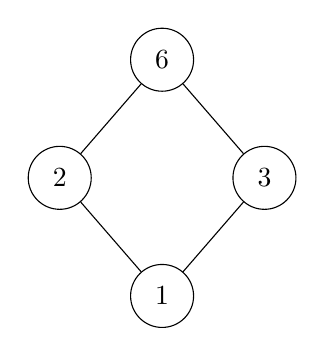
\begin{tikzpicture}[scale=1,
every node/.style={circle,draw,minimum size=8mm}]

\node (1) at (0,0) {$1$};
\node (2) at (-1.3,1.5) {$2$};
\node (3) at (1.3,1.5) {$3$};
\node (6) at (0,3) {$6$};

\draw (1)--(2);
\draw (1)--(3);
\draw (2)--(6);
\draw (3)--(6);

\end{tikzpicture}

\vspace{0.3cm}

\textbf{Hasse Diagram:} The diagram shows the divisibility order after
removing reflexive and transitive edges.

\end{frame}
%-------------------------------------------------
\begin{frame}{Example 2: Subset Relation}

\small

Let

\[
A=\{a,b\}
\]

The power set of $A$ is

\[
P(A)=
\{\emptyset,\{a\},\{b\},\{a,b\}\}
\]

Define the relation

\[
XRY \iff X\subseteq Y
\]

where "$\subseteq$" means "is a subset of".

Since the subset relation is reflexive, antisymmetric and transitive,

\[
(P(A),\subseteq)
\]

is a partially ordered set.

\end{frame}

%-------------------------------------------------
\begin{frame}{Hasse Diagram for $(P(A),\subseteq)$}

\small

\centering

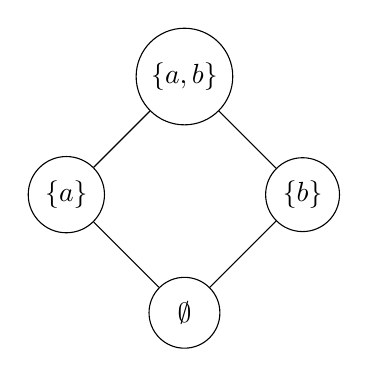
\begin{tikzpicture}[scale=1,
every node/.style={draw,circle,minimum size=9mm}]

\node (e) at (0,0) {$\emptyset$};
\node (a) at (-1.5,1.5) {$\{a\}$};
\node (b) at (1.5,1.5) {$\{b\}$};
\node (ab) at (0,3) {$\{a,b\}$};

\draw (e)--(a);
\draw (e)--(b);
\draw (a)--(ab);
\draw (b)--(ab);

\end{tikzpicture}

\vspace{0.3cm}

\textbf{Observation}

The Hasse diagram represents the subset ordering of the power set.
Only the covering relations are shown.

\end{frame}
%-------------------------------------------------
\begin{frame}{Example 3: AI Model Hierarchy}

\small

Let

\[
A=\{\text{AI},\text{Machine Learning},
\text{Deep Learning},\text{CNN},\text{RNN}\}
\]

Define the relation

\[
xRy \iff x \text{ is a subtype of } y.
\]

Examples:

\[
\text{CNN}\;R\;\text{Deep Learning}
\]

\[
\text{RNN}\;R\;\text{Deep Learning}
\]

\[
\text{Deep Learning}\;R\;\text{Machine Learning}
\]

\[
\text{Machine Learning}\;R\;\text{AI}
\]

Hence, $(A,R)$ is a partially ordered set.

\end{frame}

%-------------------------------------------------
\begin{frame}{Hasse Diagram for AI Model Hierarchy}

\small

\centering

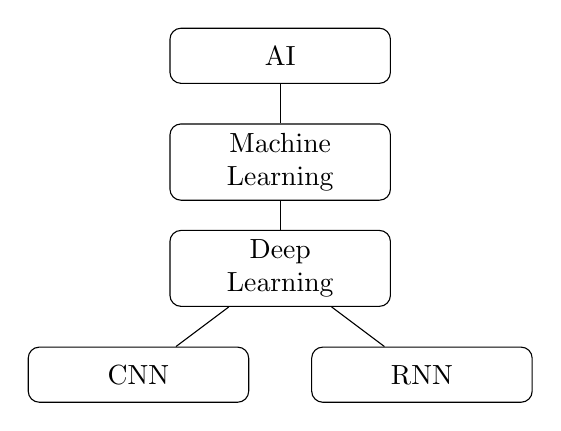
\begin{tikzpicture}[
scale=0.9,
every node/.style={
draw,
rounded corners,
minimum width=2.8cm,
minimum height=7mm,
align=center
}
]

\node (AI) at (0,4.5) {AI};

\node (ML) at (0,3) {Machine\\Learning};

\node (DL) at (0,1.5) {Deep\\Learning};

\node (CNN) at (-2,0) {CNN};

\node (RNN) at (2,0) {RNN};

\draw (CNN)--(DL);
\draw (RNN)--(DL);
\draw (DL)--(ML);
\draw (ML)--(AI);

\end{tikzpicture}

\vspace{0.3cm}

\textbf{Observation}

The diagram shows the hierarchy of AI models. CNN and RNN are incomparable,
but both are covered by Deep Learning.

\end{frame}
%-------------------------------------------------
%-------------------------------------------------
\begin{frame}{Chains and Antichains}

\small

\textbf{Chain}

A chain is a subset of a poset in which every pair of elements is comparable.

\textbf{Example:}

\[
\text{CNN}<\text{Deep Learning}
<\text{Machine Learning}<\text{AI}
\]

\[
\{\text{CNN},\text{Deep Learning},\text{Machine Learning},\text{AI}\}
\]

is a chain.

\vspace{0.2cm}

\textbf{Antichain}

An antichain is a subset of a poset in which no two distinct elements
are comparable.

\textbf{Example:}

CNN and RNN are both deep learning models, but neither is a subtype
of the other.

\[
\{\text{CNN},\text{RNN}\}
\]

is an antichain.

\end{frame}
%-------------------------------------------------
\begin{frame}{Chain and Antichain -- Hasse Diagram}

\small

\centering

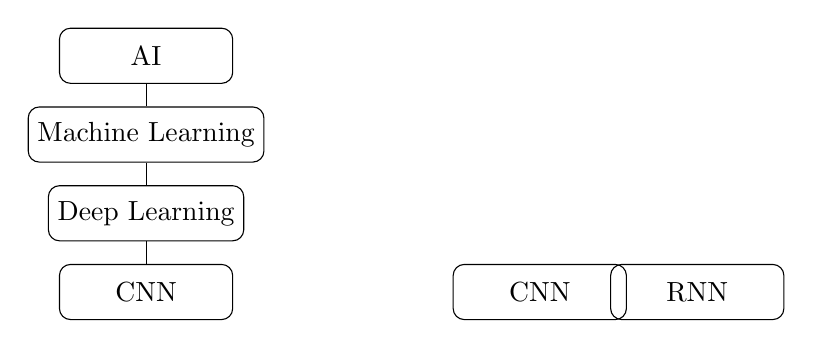
\begin{tikzpicture}[
    every node/.style={
        draw,
        rounded corners,
        minimum width=2.2cm,
        minimum height=7mm
    }
]

% Chain
\node (AI) at (0,4) {AI};
\node (ML) at (0,3) {Machine Learning};
\node (DL) at (0,2) {Deep Learning};
\node (CNN) at (0,1) {CNN};

\draw (CNN)--(DL);
\draw (DL)--(ML);
\draw (ML)--(AI);

% Antichain
\node (CNN2) at (5,1) {CNN};
\node (RNN2) at (7,1) {RNN};

\end{tikzpicture}

\vspace{0.3cm}

\begin{columns}

\column{0.48\textwidth}
\centering
\textbf{Chain}

Every pair is comparable.

\[
CNN < DL < ML < AI
\]

\column{0.48\textwidth}
\centering
\textbf{Antichain}

No two distinct elements are comparable.

\[
\{CNN,RNN\}
\]

\end{columns}

\end{frame}


\end{document}